\documentclass[11pt]{beamer}
\usetheme{Madrid}
\usefonttheme{serif}

\usepackage[utf8]{inputenc}
\usepackage[brazil]{babel}
\usepackage[T1]{fontenc}

\usepackage{amsmath}
\usepackage{amsfonts}
\usepackage{amssymb}
\usepackage{graphicx}
\usepackage{subcaption}

\DeclareMathOperator{\sen}{sen}
\DeclareMathOperator{\tg}{tg}

\setbeamertemplate{caption}[numbered]

\author[Julia G. M.; Vinícius S. F.]{\texorpdfstring{Julia Guazzelli Monteiro -- 15465383 \\ Vinícius de Sá Ferreira -- 15491650 \\ Docente: Prof. Antonio Castelo Filho}{PDFstring}}
\title{Temperaturas em Manhattan}

\setbeamertemplate{navigation symbols}{} 
\logo{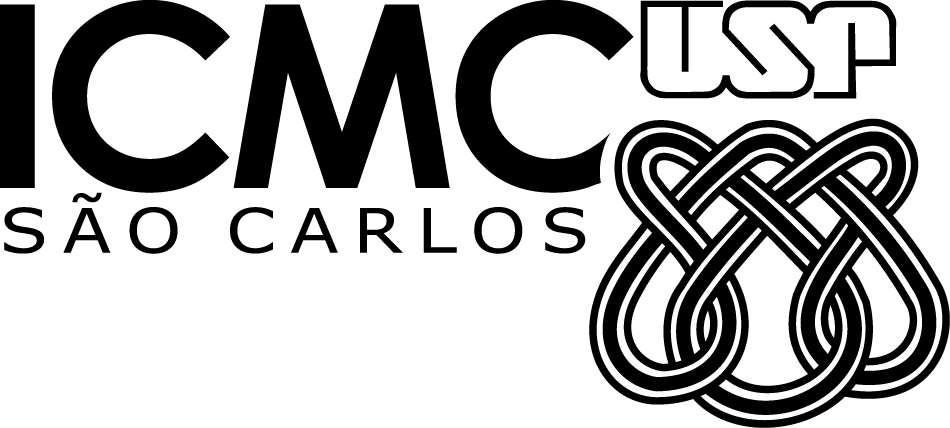
\includegraphics[scale=0.08]{icmc.png}}
\institute[]{UNIVERSIDADE DE SÃO PAULO \par MÉTODOS DE CÁLCULO NUMÉRICO I} 
\date{\today} 

\bibliographystyle{apalike}

\begin{document}

\begin{frame}
\titlepage
\end{frame}

\begin{frame}{Sumário}
    \tableofcontents 
\end{frame}

\section{Modelagem do Problema}

\begin{frame}{Modelagem do problema}
    \[\frac{\partial T(x,t)}{\partial t} = \alpha \frac{\partial^2 T(x,t)}{\partial x^2}\]
    \[T(x+1) = T(x) + T'(x) + \frac{T''(x)}{2} + \frac{T^{(3)}(x)}{6} + \frac{T^{(4)}(x)}{24} + \cdots\]
    \[T(x-1) = T(x) - T'(x) + \frac{T''(x)}{2} - \frac{T^{(3)}(x)}{6} + \frac{T^{(4)}(x)}{24} - \cdots\]
    \[T(x+1)+T(x-1) = 2T(x) + T''(x) + \frac{T^{(4)}(x)}{12} + \cdots\]
    \[T''(x) = T(x+1)-2T(x)+T(x-1) \color{gray}{- \mathcal{O}(1)}\]
    \[\frac{dT_i(t)}{dt} = \alpha (T_{i+1}(t)-2T_i(t)+T_{i-1}(t))\]
\end{frame}

\begin{frame}{Modelagem do problema}
    \scriptsize
    \[LT = \left( \left[ \begin{array}{cccc}
        G_1 & 0 & \cdots & 0\\
        0 & G_2 & \cdots & 0\\
        0 & 0 & \cdots & 0\\
        \vdots & \vdots & \ddots & \vdots\\
        0 & 0 & \cdots & G_n
    \end{array} \right] - \left[ \begin{array}{ccccc}
        &&&&\\
        &&&&\\[.19cm]
        &&A&&\\
        &&&&\\[.19cm]
        &&&&\\
    \end{array} \right] \right)_{n \times n}\left[ \begin{array}{c}
        T_1\\
        T_2\\
        T_3\\
        \vdots\\
        T_n
    \end{array} \right]_{n \times 1} = \left[ \begin{array}{c}
        C_1\\
        C_2\\
        C_3\\
        \vdots\\
        C_n
    \end{array} \right]_{n \times 1}\]
    \normalsize
    \[C_i = G_i T_i - \sum_{j \to i} T_j\]
    \[\frac{dT_i(t)}{dt} = -\alpha C_i = -\alpha (LT)_i\]
    \[\frac{dT}{dt} = -\alpha LT\]
    \[0 = \alpha LT \iff \alpha LT = b \iff (L+P)T = Pb\]
\end{frame}

\section{Métodos diretos}

\begin{frame}{Métodos Diretos}
    \[\begin{array}{ll}
        \text{Cholesky:} & M = L\cdot L^T \longrightarrow {\cal{O}}\left(\dfrac{1}{3}n^3\right)\\
        & M\cdot T = c\\
        & (L\cdot L^T)\cdot T = c\ \left\{ \begin{array}{l}
            y = L^T \cdot T\\
            L\cdot y = c
        \end{array} \right.
    \end{array}\]

    \phantom{}

    \[\begin{array}{ll}
        \text{LU:} & P\cdot M = L\cdot U \longrightarrow {\cal{O}}\left(\dfrac{2}{3}n^3\right)\\
        & M\cdot T = c\\
        & P \cdot M\cdot T = P \cdot c\\
        & (L \cdot U)\cdot T = P \cdot c\ \left\{ \begin{array}{l}
            y = U \cdot T\\
            L\cdot y = P \cdot c
        \end{array} \right.
    \end{array}\]
\end{frame}

\begin{frame}{Métodos Diretos}
    \[\begin{array}{ll}
        \text{QR:} & M = Q\cdot R \longrightarrow {\cal{O}}\left(\dfrac{4}{3}n^3\right)\\
        & M\cdot T = c\\
        & (Q\cdot R)\cdot T = c\\
        & Q^T \cdot (Q\cdot R\cdot T) = Q^T \cdot c\\
        & (Q^T \cdot Q) \cdot R\cdot T = Q^T \cdot c\\
        & R \cdot T = Q^T \cdot c
    \end{array}\]
\end{frame}

\subsection{Tempos}

\begin{frame}{Tempos}
    Quando fixamos 9 pontos dentre os 8708, obtemos
    \begin{figure}[htb]
        \label{fig:tempos_diretos_9pontos}
        \centering
        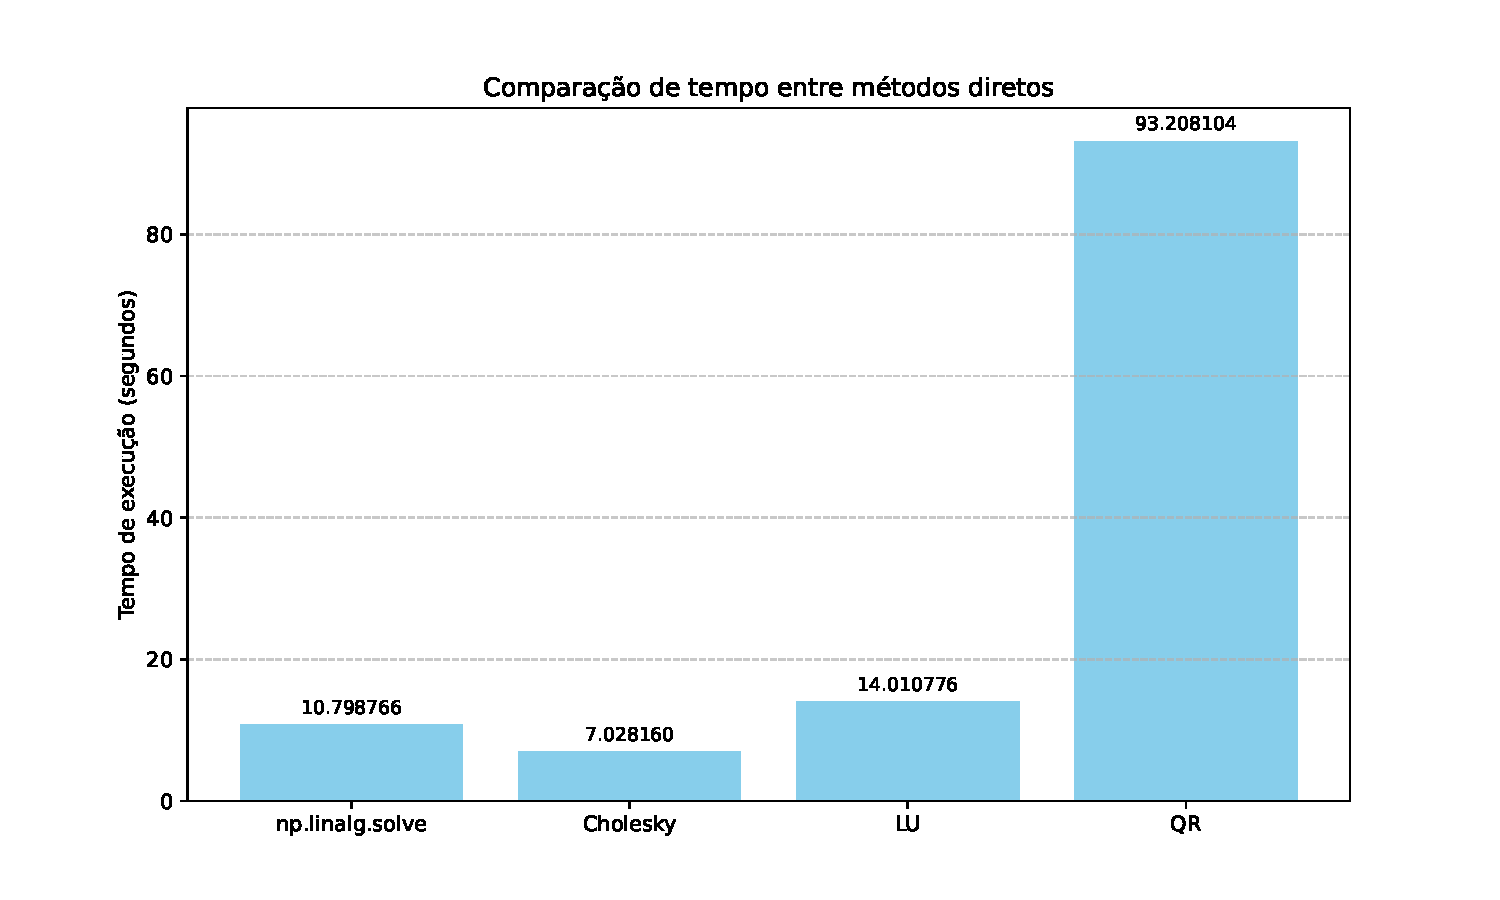
\includegraphics[width=0.9\textwidth]{../figs/fig5.pdf}
    \end{figure}
\end{frame}

\begin{frame}{Tempos}
    Quando fixamos 435 pontos dentre os 8708, obtemos
    \begin{figure}[htb]
        \label{fig:tempos_diretos_435pontos}
        \centering
        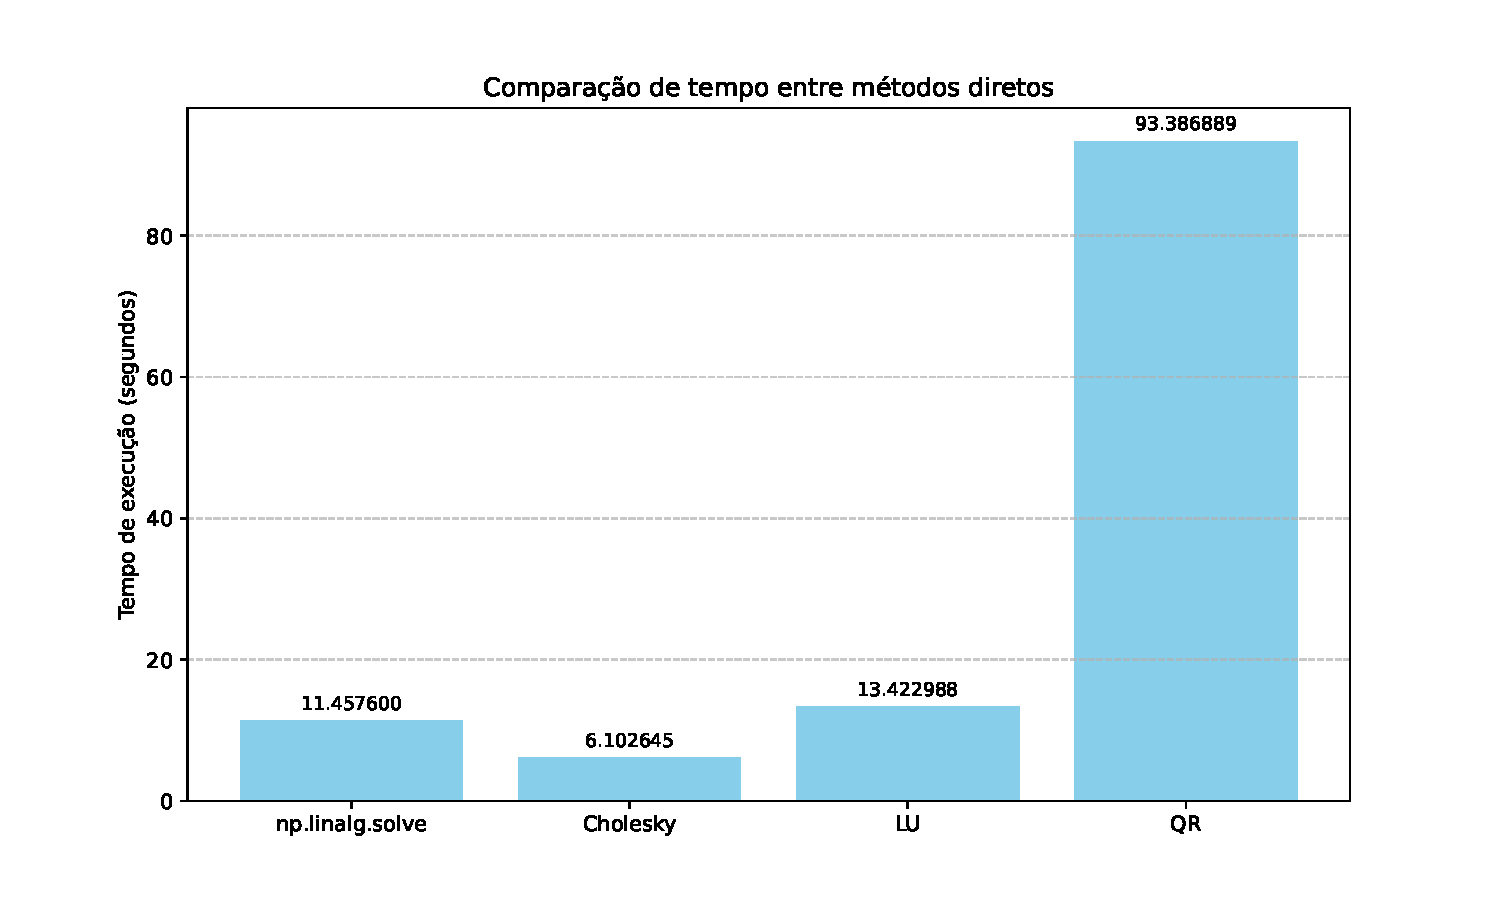
\includegraphics[width=0.9\textwidth]{../figs/fig11.pdf}
    \end{figure}
\end{frame}

\subsection{Erros}

\begin{frame}{Erros}
    Quando fixamos 9 pontos dentre os 8708, obtemos
    \begin{figure}[htb]
        \label{fig:erros_diretos_9pontos}
        \centering
        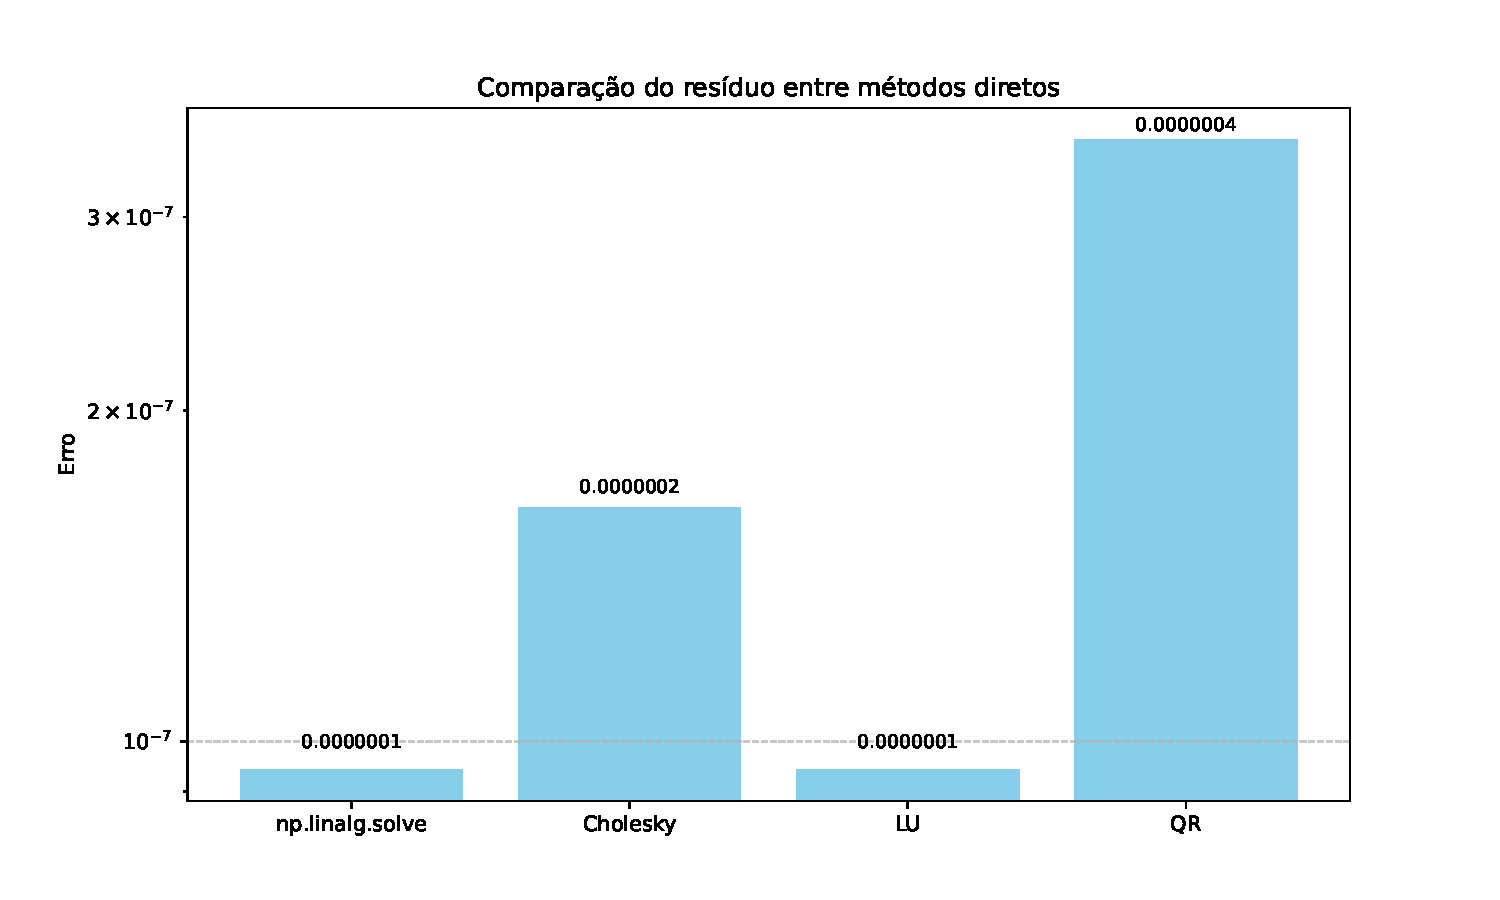
\includegraphics[width=0.9\textwidth]{../figs/fig8.pdf}
    \end{figure}
\end{frame}

\begin{frame}{Erros}
    Quando fixamos 435 pontos dentre os 8708, obtemos
    \begin{figure}[htb]
        \label{fig:erros_diretos_435pontos}
        \centering
        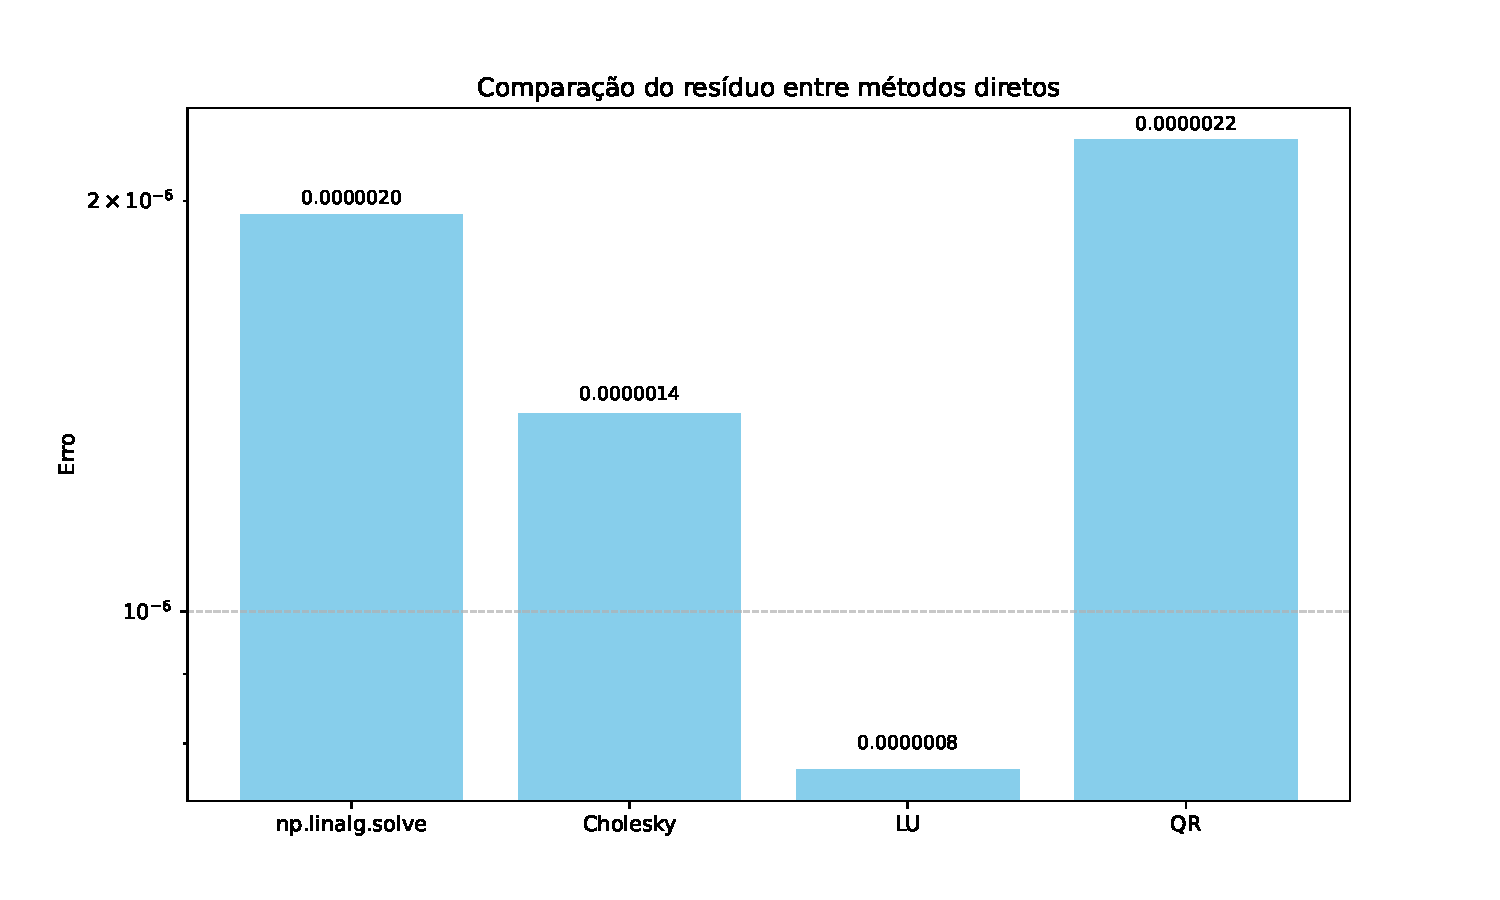
\includegraphics[width=0.9\textwidth]{../figs/fig14.pdf}
    \end{figure}
\end{frame}

\section{Métodos iterativos}

\begin{frame}{Métodos iterativos}
    Se fizermos $D$ a matriz diagonal de $M$, temos
    \[\begin{array}{ll}
        \text{Gauss-Jacobi:} & M \cdot T = c\\
        & (M - D + D)\cdot T = c\\
        & (M - D)\cdot T + D\cdot T = c\\
        & (M - D)\cdot T^{(k)} + D\cdot T^{(k+1)} = c\\
        & D\cdot T^{(k+1)} = (D - M)\cdot T^{(k)} + c\\
        & T^{(k+1)} = D^{-1}\cdot (D - M)\cdot T^{(k)} + D^{-1}\cdot c\\
        & T^{(k+1)} = (I - D^{-1}\cdot M)\cdot T^{(k)} + D^{-1}\cdot c\\
        & T^{(k+1)} = C\cdot T^{(k)} + g
    \end{array}\]
\end{frame}

\begin{frame}{Métodos iterativos}
    Se fizermos $L$ a matriz diagonal inferior de $M$ e $R$, a triangular superior sem a diagonal, temos
    \[\begin{array}{ll}
        \text{Gauss-Seidel:} & M \cdot T = c\\
        & (L+R)\cdot T = c\\
        & L\cdot T + R\cdot T = c\\
        & L\cdot T^{(k+1)} + R\cdot T^{(k)} = c\\
        & L\cdot T^{(k+1)} = -R\cdot T^{(k)} + c\\
        & T^{(k+1)} = (-L^{-1}\cdot R)\cdot T^{(k)} + L^{-1}\cdot c\\
        & T^{(k+1)} = C\cdot T^{(k)} + g
    \end{array}\]
\end{frame}

\begin{frame}{Métodos iterativos}
    \[\renewcommand{\arraystretch}{1.6}
    \begin{array}{ll}
        \text{Gradientes Conjugados:} & \text{\footnotesize 1. Chute inicial $x_0$;}\\
        & \text{\footnotesize 2. $p_0 = r_0 = c - Mx_0$;}\\
        & \text{\footnotesize 3. $\alpha = \dfrac{r_k^T \cdot r_k}{p_k^T \cdot M \cdot p_k}$;}\\
        f(x) = \dfrac{1}{2}x^TMx - c^Tx & \text{\footnotesize 4. $x_{k+1} = x_k + \alpha p_k$;}\\
        \nabla f(x) = Mx - c & \text{\footnotesize 5. $r_{k+1} = r_k - \alpha (M \cdot p_k)$;}\\
        & \text{\footnotesize 6. $\beta = \dfrac{r_{k+1}^T \cdot r_{k+1}}{r_k^T \cdot r_k}$;}\\
        & \text{\footnotesize 7. $p_{k+1} = r_{k+1} + \beta p_k$;}\\
        & \text{\footnotesize 8. Volta para o passo 3, enquanto $\|r_{k+1}\| > $ tol.}\\
    \end{array}\]
\end{frame}

\subsection{Tempos}

\begin{frame}{Tempos}
    Quando fixamos 9 pontos dentre os 8708 e uma tolerância de $10^{-1}$, obtemos
    \begin{figure}[htb]
        \label{fig:tempos_iterativos_9pontos}
        \centering
        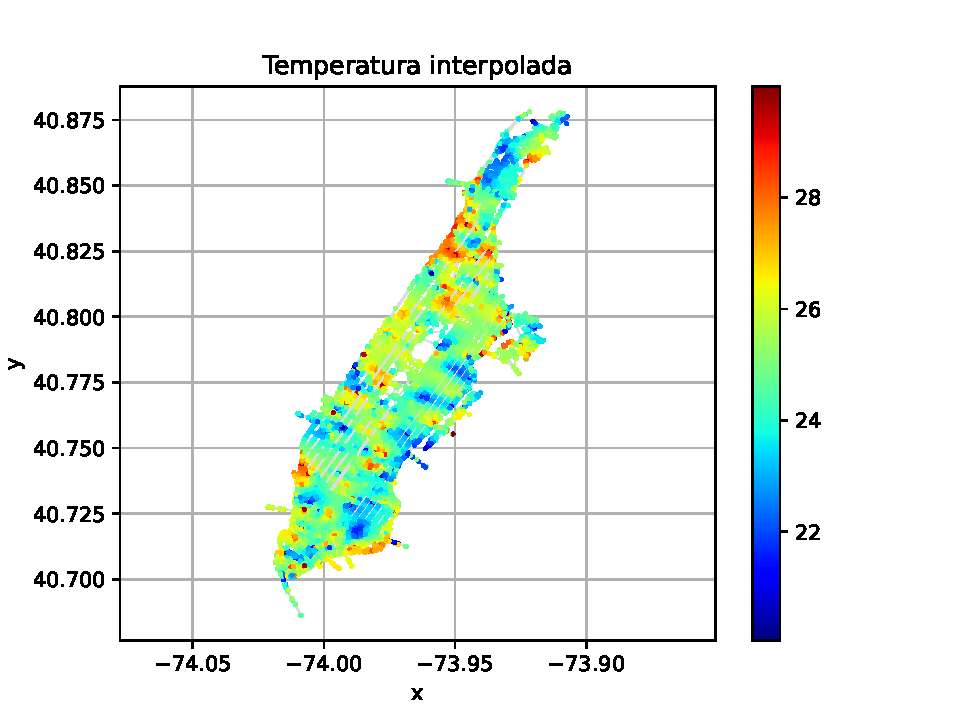
\includegraphics[width=0.9\textwidth]{../figs/fig6.pdf}
    \end{figure}
\end{frame}

\begin{frame}{Tempos}
    Quando fixamos 435 pontos dentre os 8708 e uma tolerância de $10^{-3}$, obtemos
    \begin{figure}[htb]
        \label{fig:tempos_iterativos_435pontos}
        \centering
        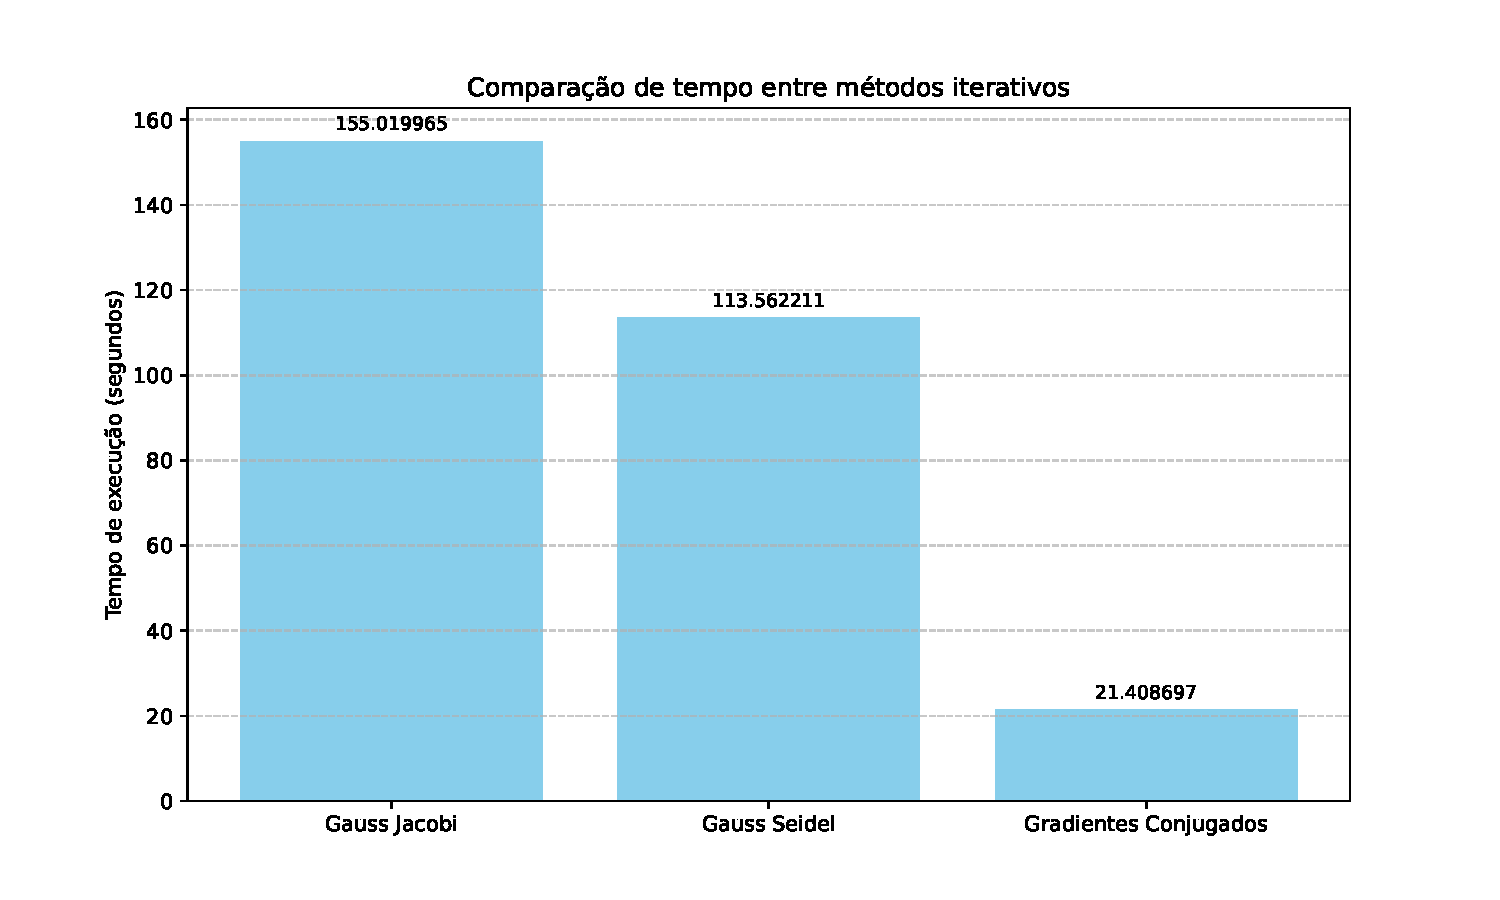
\includegraphics[width=0.9\textwidth]{../figs/fig12.pdf}
    \end{figure}
\end{frame}

\begin{frame}{Tempos}
    Obtivemos também a quantidade de passos necessários para convergir

    \footnotesize
    \[\renewcommand{\arraystretch}{1.5}
    \begin{array}{|c|c|c|c|c|c|}
        \hline
        \text{Pontos} & \text{Tolerância} & & \text{Gauss-Jacobi} & \text{Gauss-Seidel} & \text{Gradientes Conjugados}\\
        \hline
        \smash{\raisebox{-.3cm}{9}} & \smash{\raisebox{-.3cm}{$10^{-1}$}} & k & 13000 & 7129 & 630\\
        \cline{3-6}
        & & \text{t} & 19\text{ min} & 11\text{ min} & 1\text{ min}\\
        \hline
        \smash{\raisebox{-.3cm}{435}} & \smash{\raisebox{-.3cm}{$10^{-3}$}} & k & 1261 & 647 & 251\\
        \cline{3-6}
        & & \text{t} & 3\text{ min} & 2\text{ min} & 30\text{ s}\\
        \hline
    \end{array}\]
\end{frame}

\subsection{Erros}

\begin{frame}{Erros}
    Quando fixamos 9 pontos dentre os 8708 e uma tolerância de $10^{-1}$, obtemos
    \begin{figure}[htb]
        \label{fig:erros_iterativos_9pontos}
        \centering
        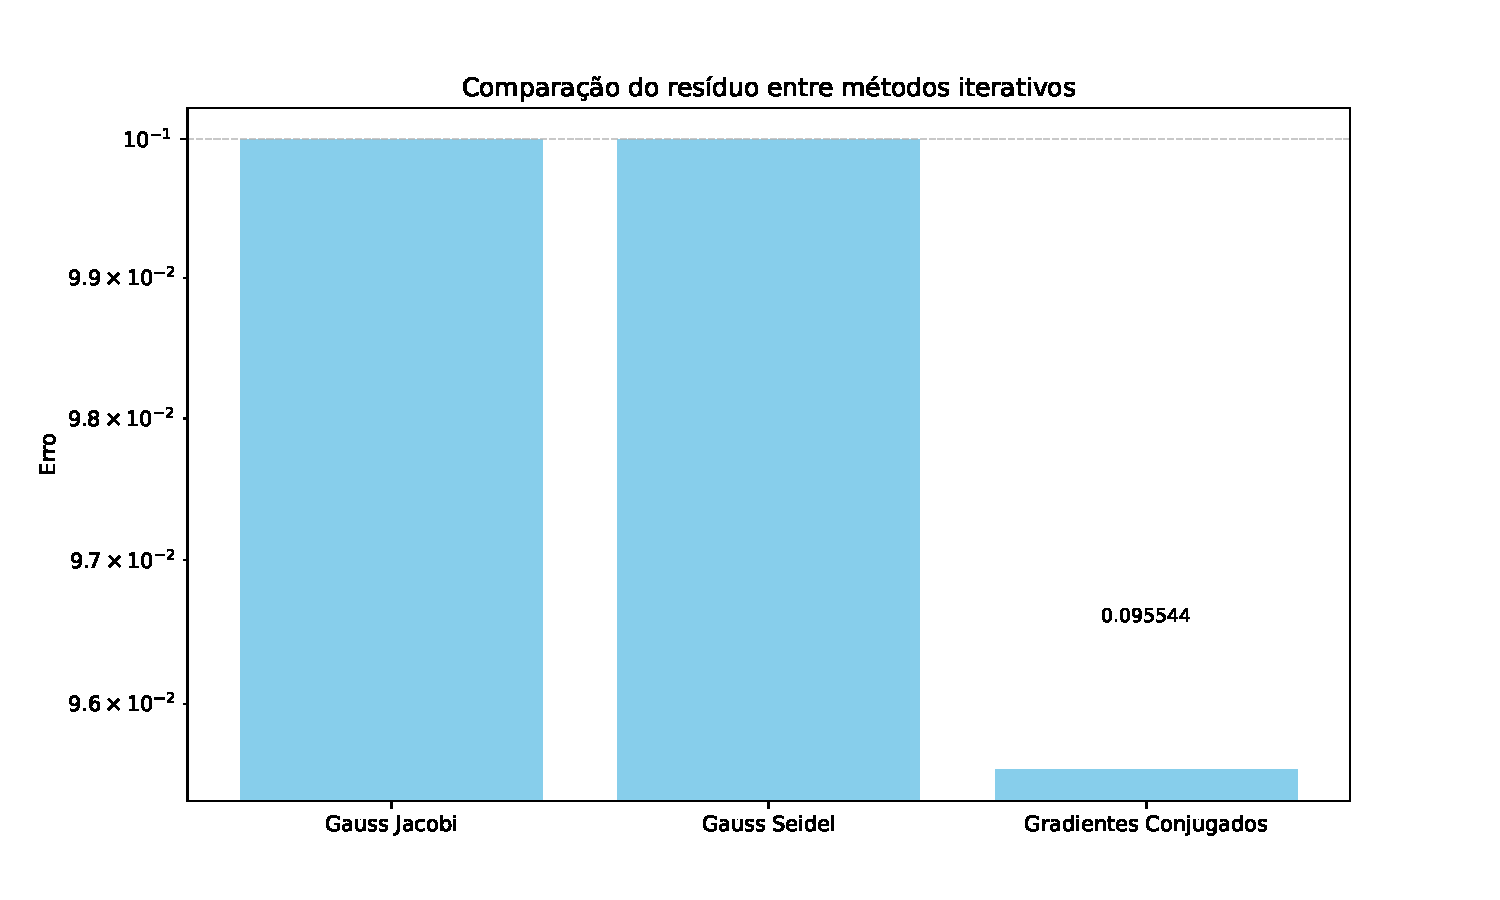
\includegraphics[width=0.9\textwidth]{../figs/fig9.pdf}
    \end{figure}
\end{frame}

\begin{frame}{Erros}
    Quando fixamos 435 pontos dentre os 8708 e uma tolerância de $10^{-3}$, obtemos
    \begin{figure}[htb]
        \label{fig:erros_iterativos_435pontos}
        \centering
        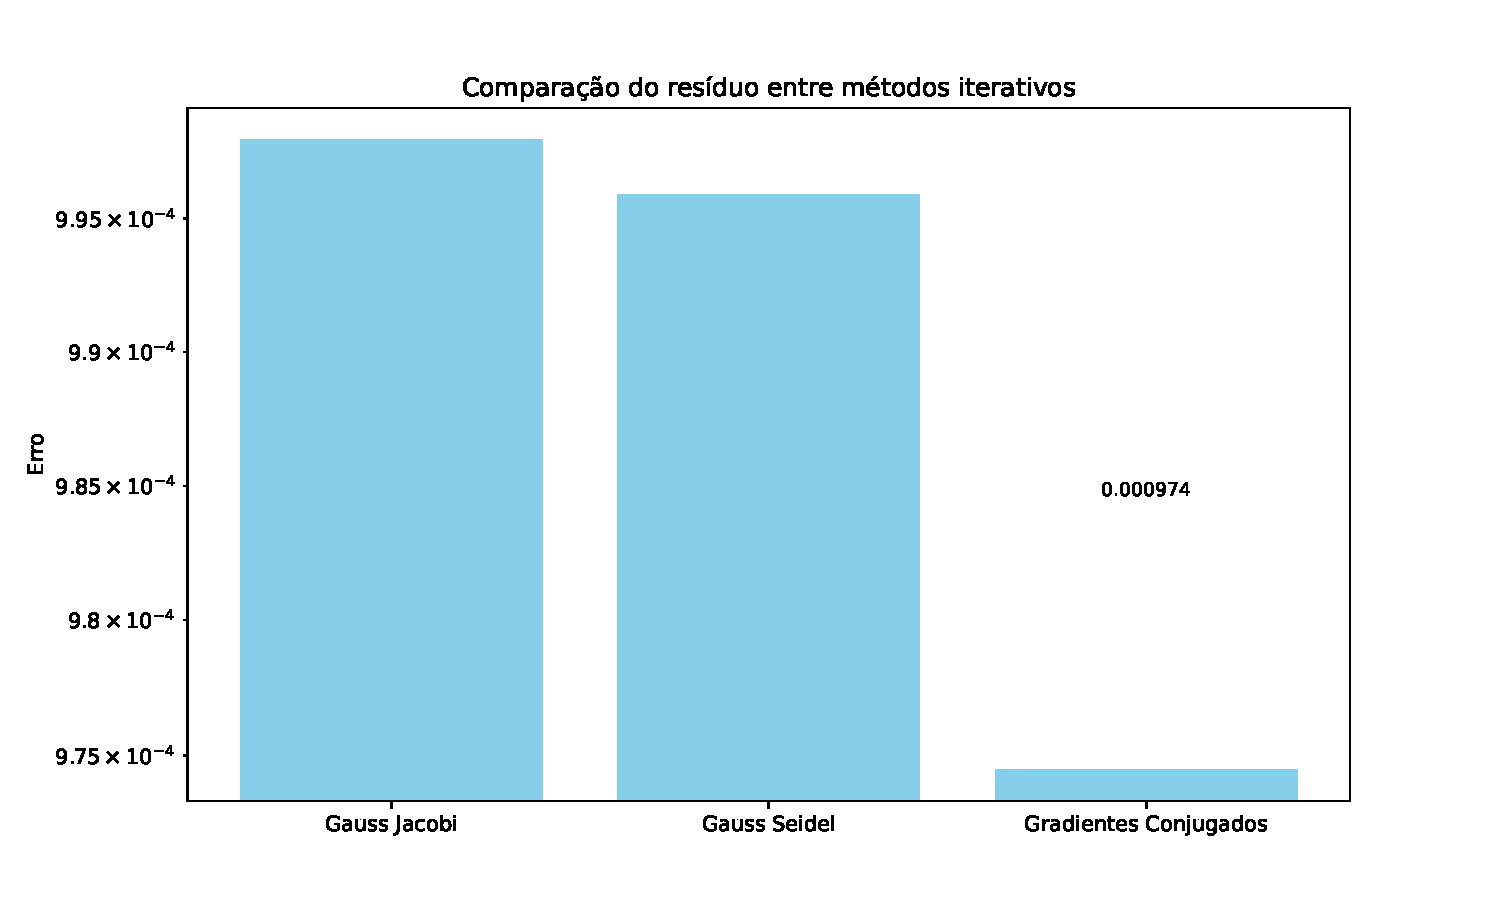
\includegraphics[width=0.9\textwidth]{../figs/fig15.pdf}
    \end{figure}
\end{frame}

\section{Resultados}

\begin{frame}{Resultados}
    \begin{figure}[htb]
        \label{fig:grafo_desconexo}
        \centering
        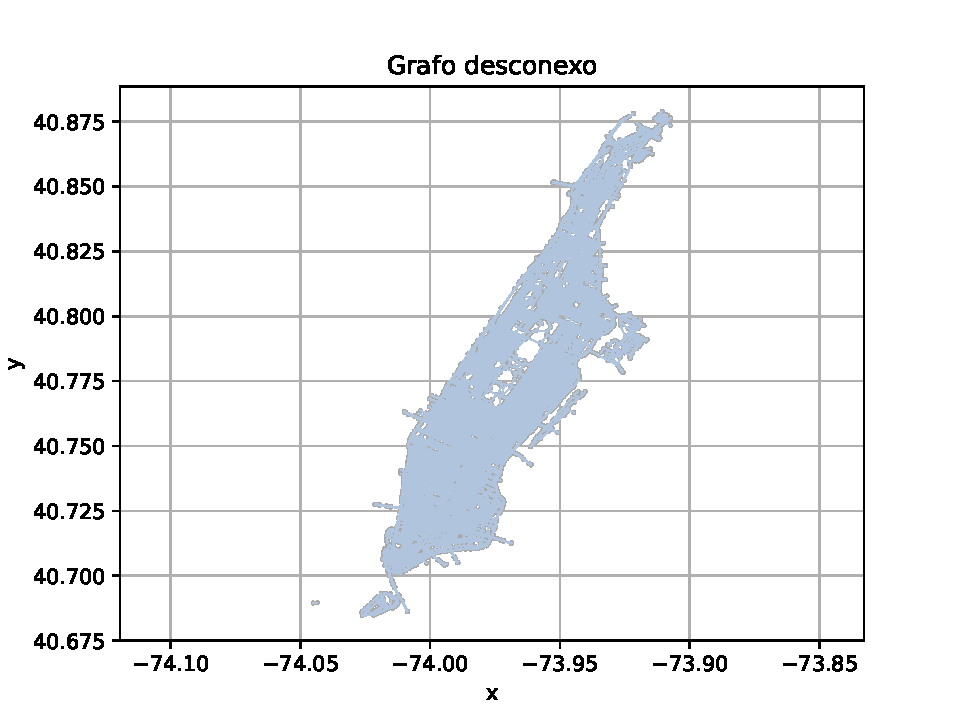
\includegraphics[width=0.8\textwidth]{../figs/fig1.pdf}
    \end{figure}
\end{frame}

\begin{frame}{Resultados}
    \begin{figure}[htb]
        \label{fig:componentes_conexas}
        \centering
        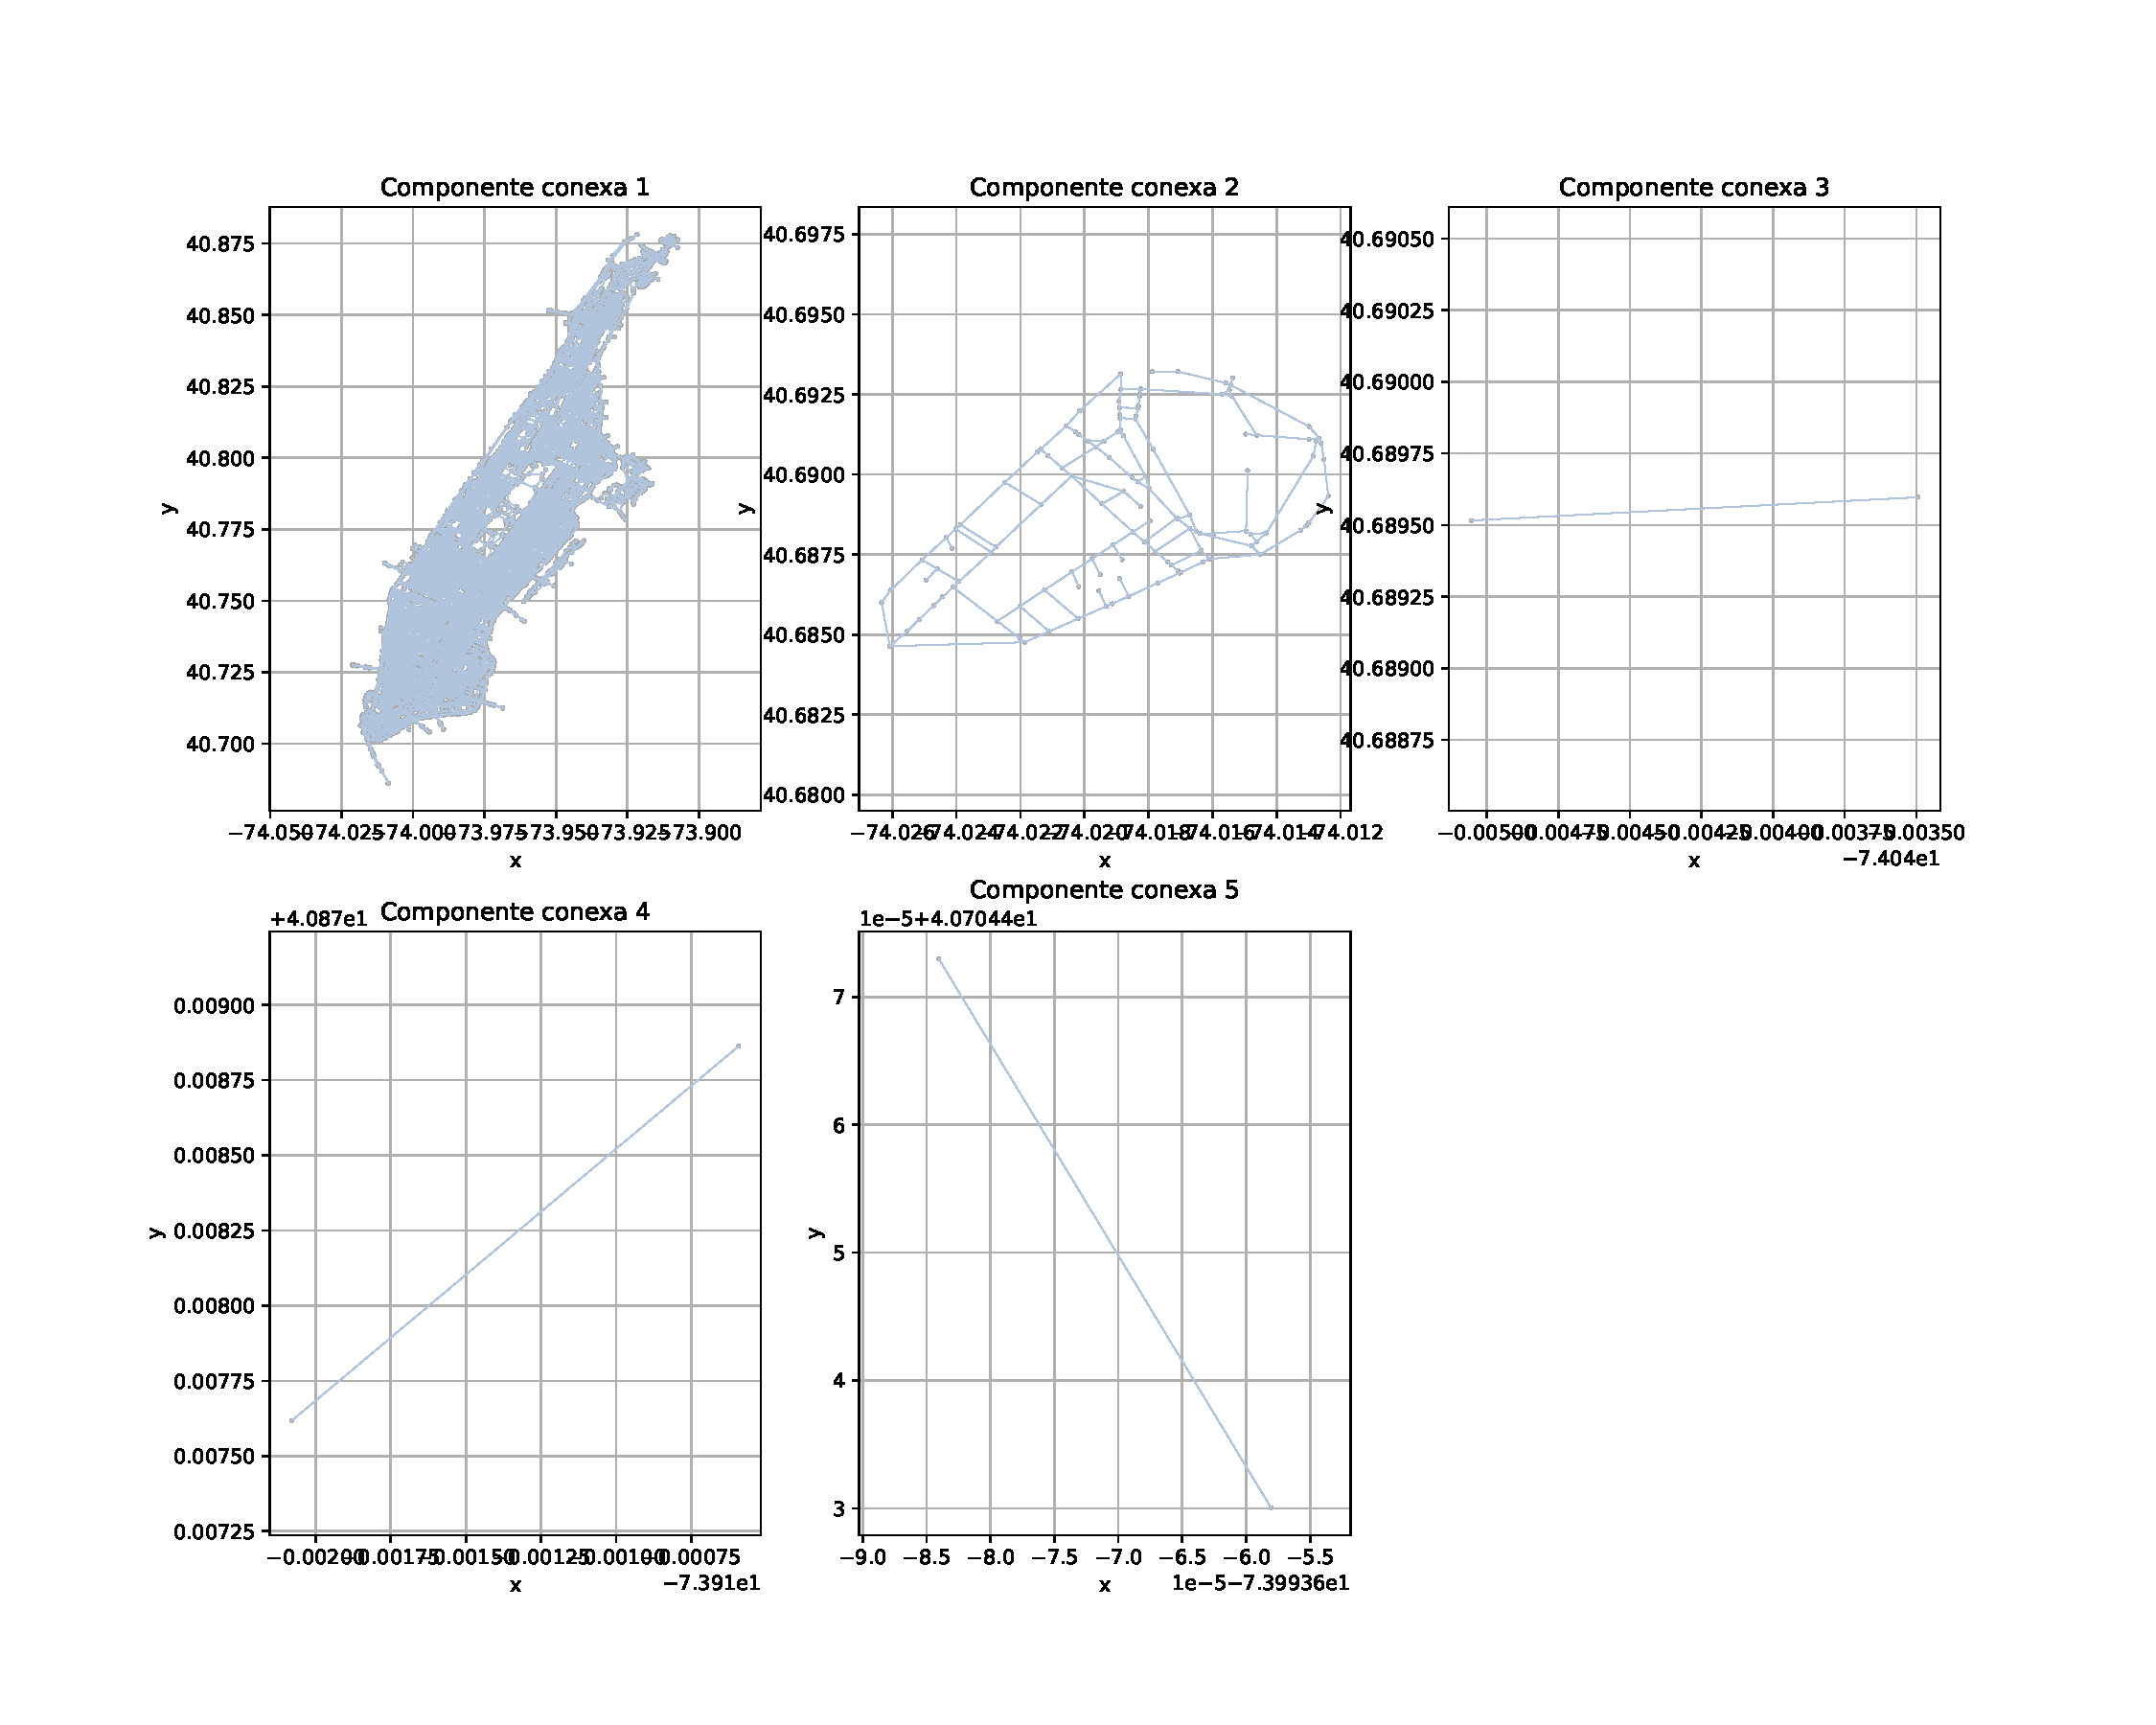
\includegraphics[width=0.9\textwidth]{../figs/fig2.pdf}
    \end{figure}
\end{frame}

\begin{frame}{Resultados}
    \begin{figure}[htb]
        \label{fig:maior_componente_conexa}
        \centering
        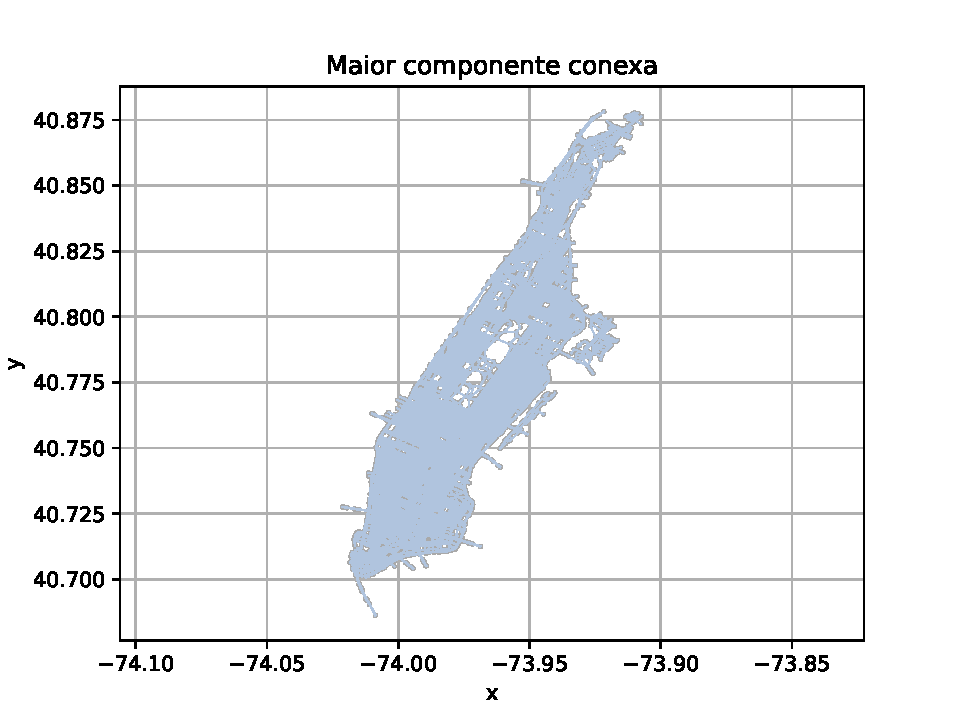
\includegraphics[width=0.8\textwidth]{../figs/fig3.pdf}
    \end{figure}
\end{frame}

\begin{frame}{Resultados}
    \begin{figure}[htb]
        \hspace{-1cm}
        \begin{subfigure}{0.4\textwidth}
            \label{fig:fixos_9pontos}
            \centering
            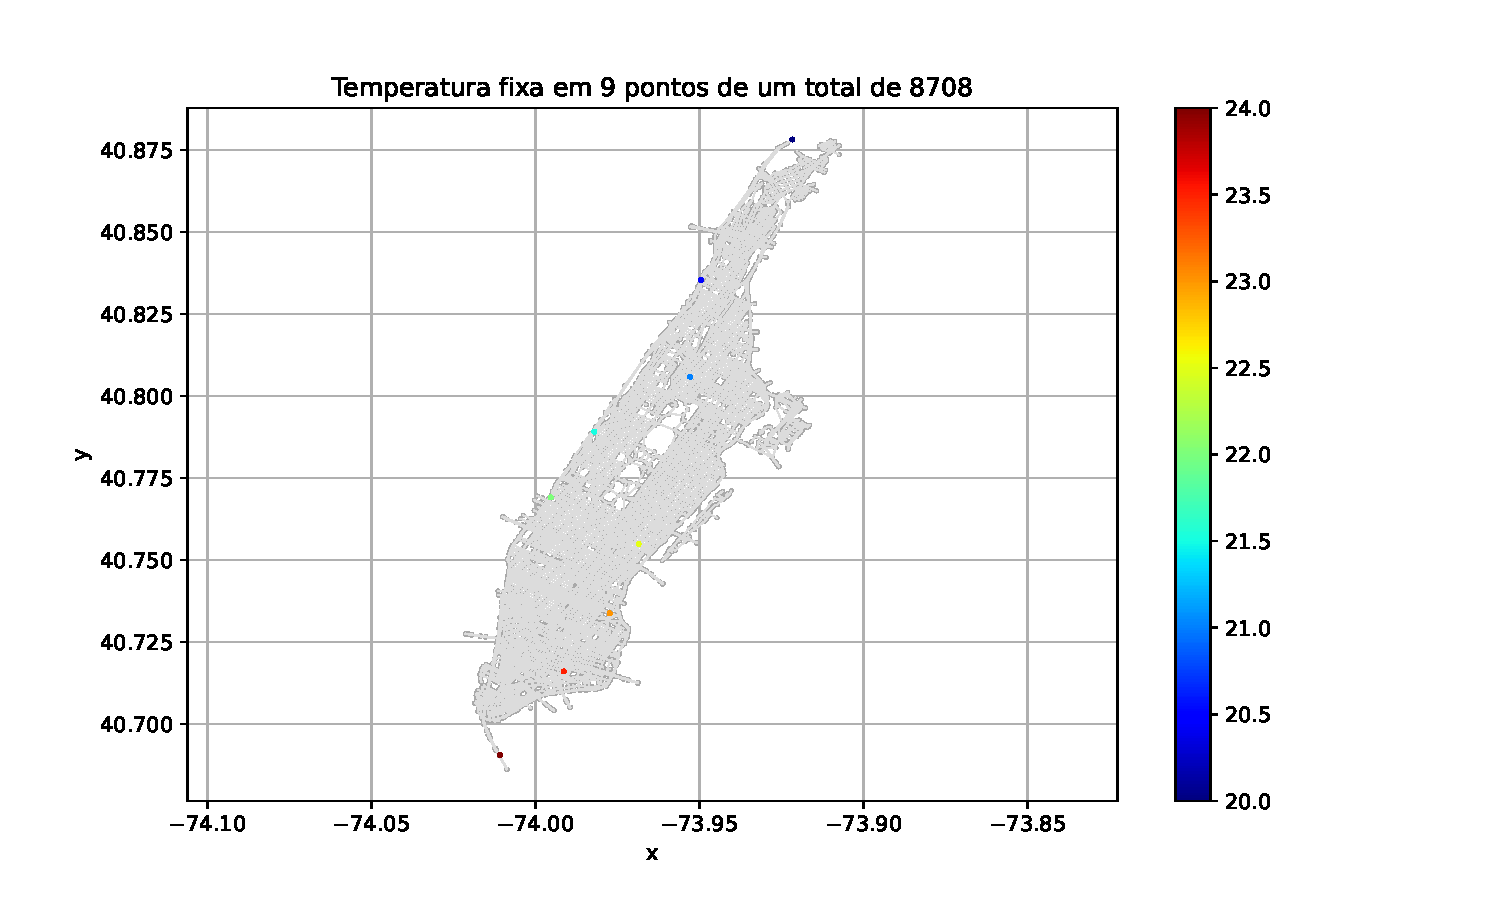
\includegraphics[height=0.95\textwidth]{../figs/fig4.pdf}
        \end{subfigure}
        \hspace{1.9cm}
        \begin{subfigure}{0.4\textwidth}
            \label{fig:interpolado_9pontos}
            \centering
            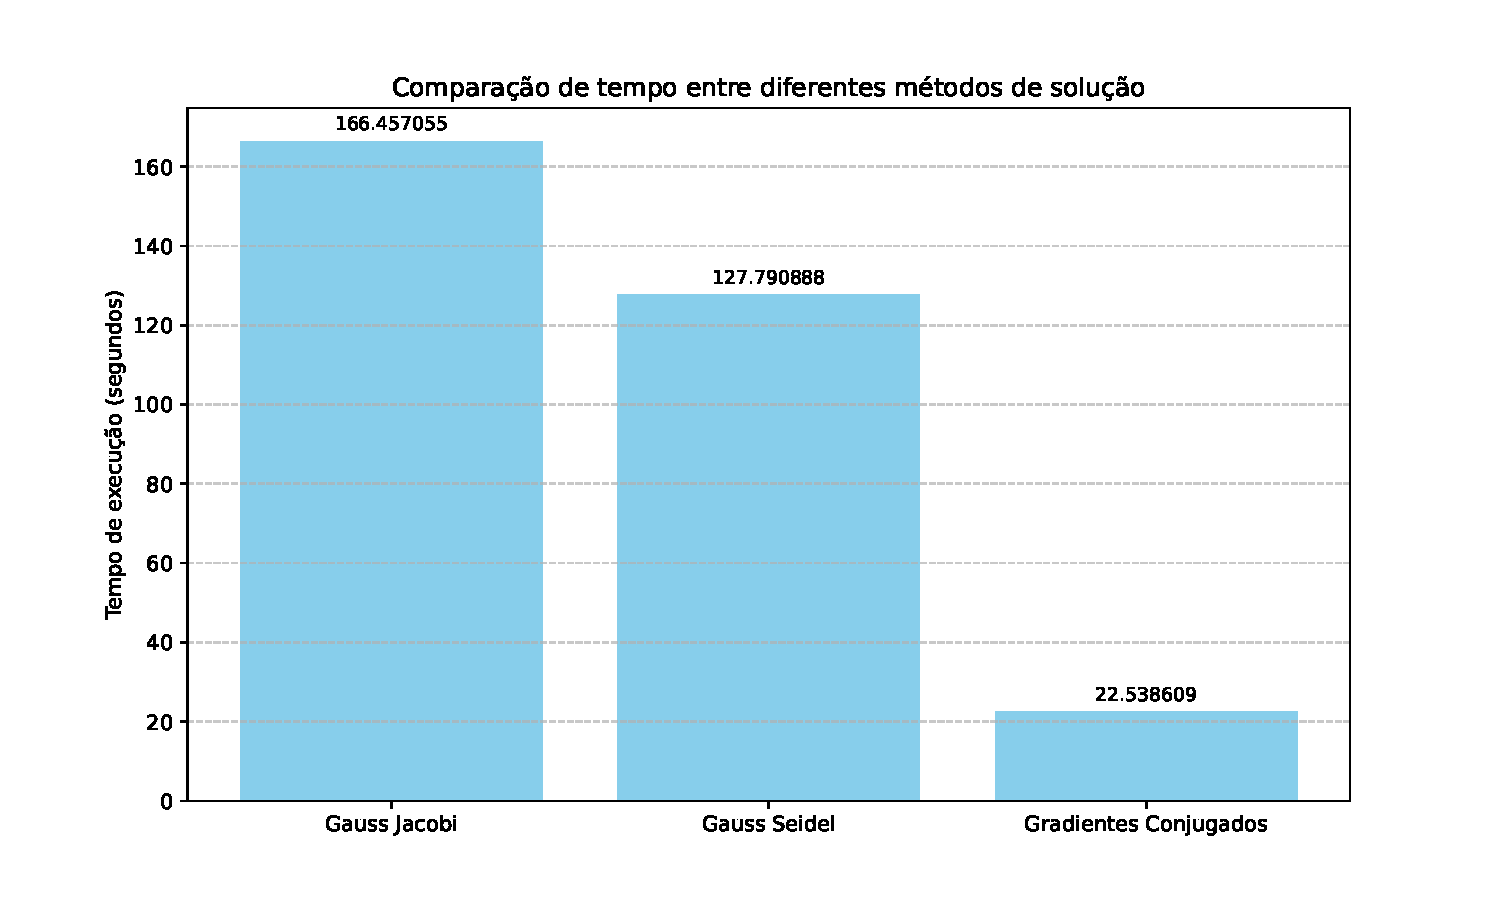
\includegraphics[height=0.95\textwidth]{../figs/fig7.pdf}
        \end{subfigure}
    \end{figure}
\end{frame}

\begin{frame}{Resultados}
    \begin{figure}[htb]
        \hspace{-1cm}
        \begin{subfigure}{0.4\textwidth}
            \label{fig:fixos_435pontos}
            \centering
            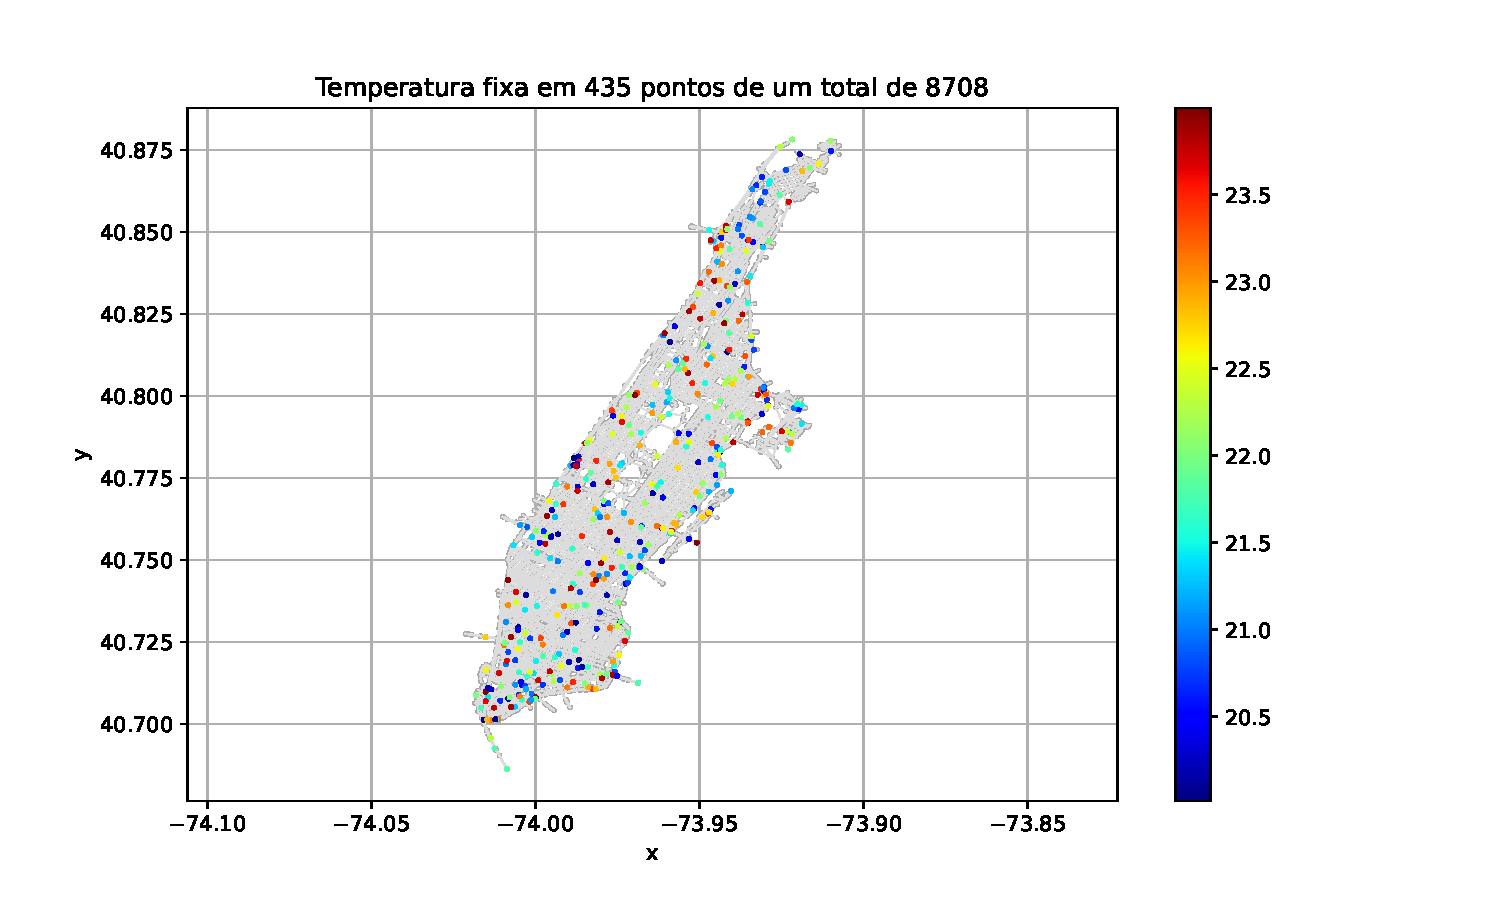
\includegraphics[height=0.95\textwidth]{../figs/fig10.pdf}
        \end{subfigure}
        \hspace{1.9cm}
        \begin{subfigure}{0.4\textwidth}
            \label{fig:interpolado_435pontos}
            \centering
            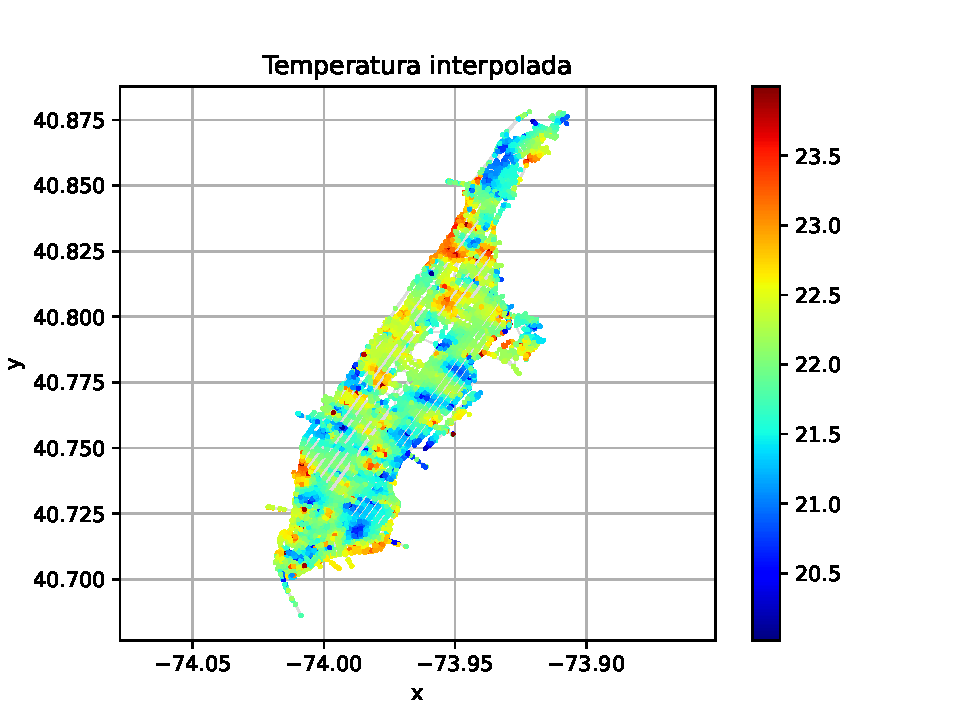
\includegraphics[height=0.95\textwidth]{../figs/fig13.pdf}
        \end{subfigure}
    \end{figure}
\end{frame}

\begin{frame}
    \begin{center}
        Dúvidas?
    \end{center}
\end{frame}

\end{document}